\begin{center}
\LARGE
Delprøve uden hjælpemidler 
\end{center}
\stepcounter{section}
%%%%%%%%%%%%%%%%%%%%%%%%%%%%%%%%%%%%%%%%%%%%%%%%%%%%%%%%%%%%%%%%%%%%%%%
%							Ny Opgave!!!!!							%
%%%%%%%%%%%%%%%%%%%%%%%%%%%%%%%%%%%%%%%%%%%%%%%%%%%%%%%%%%%%%%%%%%%%%%%
\begin{opgavetekst}{Opgave 1}
	En stokastisk variabel $X$ har sandsynlighedsfunktion $P$ og udfaldsrum  \\
	$U = \{a,b,c,d,e\}$. Fordelingen for $X$ 
	kan ses af Tab. \ref{tab:fordeling}.
	\begin{table}[H]
		\centering
		\begin{tabular}{c|c|c|c|c|c}
			$U$ & $a$ & $b$ &  $c$ & $d$ & $e$ \\
			\hline
			$P(X=x)$ & 0.5 & 0.1 & 0.05 & 0.05 & $P(X=e)$
		\end{tabular}
		\caption{Fordeling for den stokastiske variabel $X$. }
		\label{tab:fordeling}		
	\end{table}
	\phantom{h}
\end{opgavetekst}
	\begin{delopgave}{}{1}
		Bestem $P(X=e)$.
	\end{delopgave}

%%%%%%%%%%%%%%%%%%%%%%%%%%%%%%%%%%%%%%%%%%%%%%%%%%%%%%%%%%%%%%%%%%%%%%%
%							Ny Opgave!!!!!							%
%%%%%%%%%%%%%%%%%%%%%%%%%%%%%%%%%%%%%%%%%%%%%%%%%%%%%%%%%%%%%%%%%%%%%%%
\begin{opgavetekst}{Opgave 2}
	Af Fig. \ref{fig:fordeling} ses fordelingsfunktionerne $F$ og $G$ for to normalfordelte stokastiske variable
	\begin{align*}
		X \sim N(\mu,1)
	\end{align*}
	og 
	\begin{align*}
		Y \sim N(\mu,1.5).
	\end{align*}
	\begin{figure}[H]
		\centering
		\includegraphics[width=0.7\textwidth]{Billeder/fordelingafl.jpg}
		\caption{Fordelingsfunktionerne $F$ og $G$.}
		\label{fig:fordeling}
	\end{figure}
	\phantom{h}
\end{opgavetekst}
	\begin{delopgave}{}{1}
		Bestem middelværdien $\mu$ for de to stokastiske variable.
	\end{delopgave}
	\begin{delopgave}{}{2}
		Hvilken af de to kurver tilsvarer fordelingsfunktionen for henholdsvist $X$ og $Y$?
	\end{delopgave}
	\begin{delopgave}{}{3}
		Bestem sandsynlighederne
		\begin{align*}
			P(2<X<4) \textnormal{ og } P(1<Y).
		\end{align*}
	\end{delopgave}
%%%%%%%%%%%%%%%%%%%%%%%%%%%%%%%%%%%%%%%%%%%%%%%%%%%%%%%%%%%%%%%%%%%%%%%
%							Ny Opgave!!!!!							%
%%%%%%%%%%%%%%%%%%%%%%%%%%%%%%%%%%%%%%%%%%%%%%%%%%%%%%%%%%%%%%%%%%%%%%%

\begin{opgavetekst}{Opgave 3}
	\begin{center}
		\includegraphics[width=0.5\textwidth]{Billeder/pizza.jpg}
	\end{center}
	For en bestemt type stafylokok-bakterie gælder det, at væksten af dem $S'$ (i mio. pr. minut) i fødevarer ved stuetemperatur er proportional med antallet af bakterier $S$ (i mio.). 
\end{opgavetekst}
\begin{delopgave}{}{1}
	Opstil en differentialligningsmodel, der beskriver væksten af stafylokokbakterien i fødevarer, når det oplyses at proportionalitetskonstanten er 0.024.
\end{delopgave}
\begin{delopgave}{}{2}
	Opskriv en partikulær løsning til differentialligningsmodellen, hvis det oplyses, at antallet af bakterier til $t=0$ er 792 mio. 
\end{delopgave}
%%%%%%%%%%%%%%%%%%%%%%%%%%%%%%%%%%%%%%%%%%%%%%%%%%%%%%%%%%%%%%%%%%%%%%%
%							Ny Opgave!!!!!							%
%%%%%%%%%%%%%%%%%%%%%%%%%%%%%%%%%%%%%%%%%%%%%%%%%%%%%%%%%%%%%%%%%%%%%%%
\begin{opgavetekst}{Opgave 4 }
	\begin{center}
		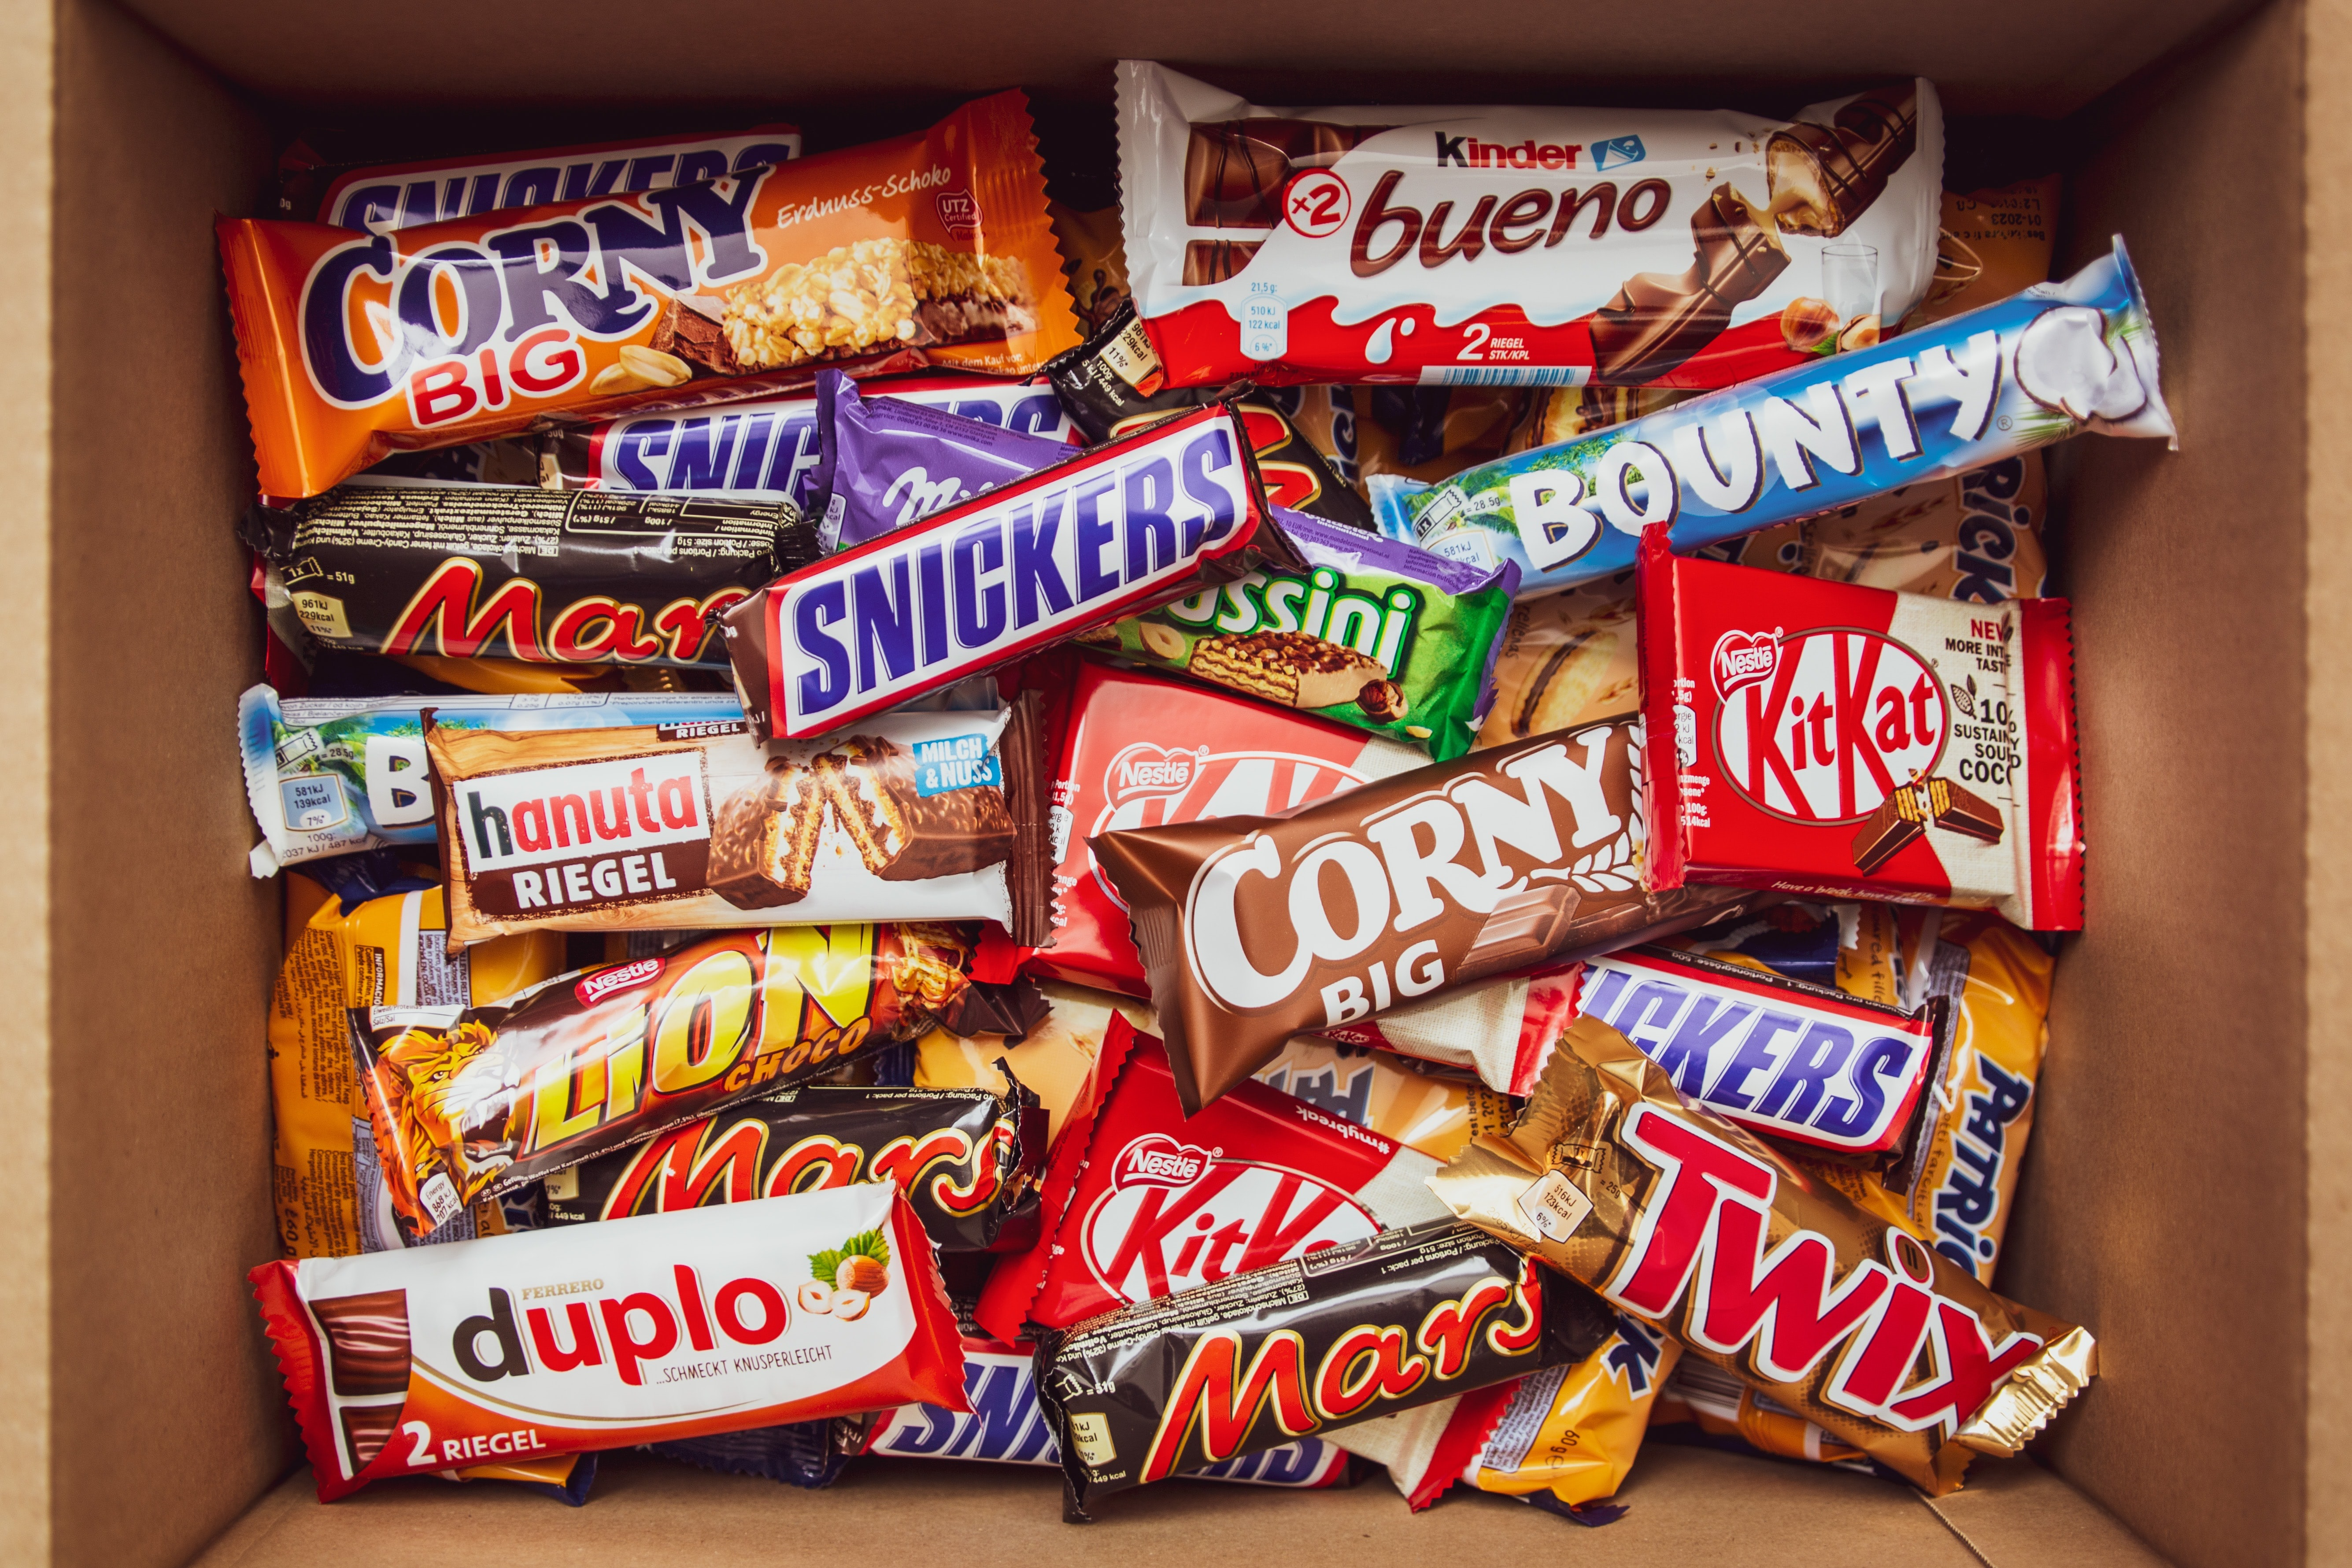
\includegraphics[width=0.7\textwidth]{Billeder/choko.jpg}
	\end{center}
	En producent af chokoladebarer har undersøgt en bestemt slags af sine chokoladebarer og opdaget, at vægten af netop dén type chokoladebar er normalfordelt
	med en middelværdi på 51g og en spredning på 4.5g.
\end{opgavetekst}
\begin{delopgave}{}{1}
	Afgør, om en chokoladebar på 57g er et normalt udfald. 
\end{delopgave}
\begin{meretekst}
	Vi lader $f$ betegne tæthedsfunktionen for den normalfordelte stokastiske variabel, der beskriver vægten af chokoladebarerne. 
\end{meretekst}
\begin{delopgave}{}{2}
	Hvad siger følgende integral om vægten af chokoladebarerne?
	\begin{align*}
		\int_{48}^{65} f(x)dx \approx  0.747.
	\end{align*}
\end{delopgave}
%%%%%%%%%%%%%%%%%%%%%%%%%%%%%%%%%%%%%%%%%%%%%%%%%%%%%%%%%%%%%%%%%%%%%%%
%							Ny Opgave!!!!!							%
%%%%%%%%%%%%%%%%%%%%%%%%%%%%%%%%%%%%%%%%%%%%%%%%%%%%%%%%%%%%%%%%%%%%%%%
\begin{opgavetekst}{Opgave 5}
	En funktion $f:\mathbb{R}^2 \to \mathbb{R}$ er givet ved
	\begin{align*}
		f(x,y) = \ln(x)\cdot(x-y) + y^2x
	\end{align*}
\end{opgavetekst}
\begin{delopgave}{}{1}
	Bestem $f(1,2)$
\end{delopgave}
\begin{delopgave}{}{2}
	Bestem $f_x'(x,y)$ og $f_y'(x,y)$
\end{delopgave}

%%%%%%%%%%%%%%%%%%%%%%%%%%%%%%%%%%%%%%%%%%%%%%%%%%%%%%%%%%%%%%%%%%%%%%%
%							Ny Opgave!!!!!							%
%%%%%%%%%%%%%%%%%%%%%%%%%%%%%%%%%%%%%%%%%%%%%%%%%%%%%%%%%%%%%%%%%%%%%%%



\newpage
\begin{center}
\LARGE
Delprøve med hjælpemidler 
\end{center}
\stepcounter{section}
%%%%%%%%%%%%%%%%%%%%%%%%%%%%%%%%%%%%%%%%%%%%%%%%%%%%%%%%%%%%%%%%%%%%%%%
%							Ny Opgave!!!!!							%
%%%%%%%%%%%%%%%%%%%%%%%%%%%%%%%%%%%%%%%%%%%%%%%%%%%%%%%%%%%%%%%%%%%%%%%


\begin{opgavetekst}{Opgave 6}
	\begin{center}
		\includegraphics[width=0.7\textwidth]{Billeder/measure.jpg}
	\end{center}
	I en by har man målt alle drenges højde på deres 12-års fødselsdag. Deres højde kan findes \href{https://github.com/ChristianJLex/TeachingNotes/raw/master/2022-2023/Data%20og%20lign/Hojde.xlsx}{\color{blue!60} her}.
\end{opgavetekst}
\begin{delopgave}{}{1}
	Vis, at datasættet er approksimativt normalfordelt og bestem middelværdien og spredningen for datasættet. 
\end{delopgave}
\begin{delopgave}{}{2}
	Bestem sandsynligheden for at en tolvårig dreng har en højde på under 140cm. 
\end{delopgave}
\begin{delopgave}{}{3}
	Er en højde på 110cm et exceptionelt udfald?
\end{delopgave}
\newpage
%%%%%%%%%%%%%%%%%%%%%%%%%%%%%%%%%%%%%%%%%%%%%%%%%%%%%%%%%%%%%%%%%%%%%%%
%							Ny Opgave!!!!!							%
%%%%%%%%%%%%%%%%%%%%%%%%%%%%%%%%%%%%%%%%%%%%%%%%%%%%%%%%%%%%%%%%%%%%%%%
\begin{opgavetekst}{Opgave 7}
	En vektorfunktion $\vv{r}: \mathbb{R} \to \mathbb{R}^2$ er givet ved
	\begin{align*}
		\vv{r}(t) = 
		\begin{pmatrix}
			2t^3-t^2+7\\
			4t^4-6t^2-t-9
		\end{pmatrix}
	\end{align*}
\end{opgavetekst}
\begin{delopgave}{}{1}
	Tegn $\vv{r}$ på parameterintervallet $[-2,2]$.
\end{delopgave}
\begin{delopgave}{}{2}
	Bestem parameterkurven for $\vv{r}$'s skæring med akserne. 
\end{delopgave}
%%%%%%%%%%%%%%%%%%%%%%%%%%%%%%%%%%%%%%%%%%%%%%%%%%%%%%%%%%%%%%%%%%%%%%%
%							Ny Opgave!!!!!							%
%%%%%%%%%%%%%%%%%%%%%%%%%%%%%%%%%%%%%%%%%%%%%%%%%%%%%%%%%%%%%%%%%%%%%%%
\begin{opgavetekst}{Opgave 8}
	Lad $f$ og $g$ være givet ved
	\begin{align*}
		f(x) = \ln(x)-x^2+10
	\end{align*}
	og 
	\begin{align*}
		g(x) = x^2-1.
	\end{align*}
\end{opgavetekst}
\begin{delopgave}{}{1}
	Tegn graferne for $f$ og $g$ på intervallet $[0,4]$.
\end{delopgave}
\begin{delopgave}{}{2}
	Bestem skæringspunkterne mellem graferne for de to funktioner. 
\end{delopgave}
\begin{meretekst}
	Graferne for de to funktioner afgrænser sammen med $x$-aksen et trekantlignende område $M$.
\end{meretekst}
\begin{delopgave}{}{3}
	Bestem arealet af $M$. 
\end{delopgave}

\newpage
%%%%%%%%%%%%%%%%%%%%%%%%%%%%%%%%%%%%%%%%%%%%%%%%%%%%%%%%%%%%%%%%%%%%%%%
%							Ny Opgave!!!!!							%
%%%%%%%%%%%%%%%%%%%%%%%%%%%%%%%%%%%%%%%%%%%%%%%%%%%%%%%%%%%%%%%%%%%%%%%

\begin{opgavetekst}{Opgave 9}
	Taget på en bestemt kvadratisk bygning er udformet, så taget tilsvarer grafen for funktionen $f:\mathbb{R}^2 \to \mathbb{R}$ givet ved
	\begin{align*}
		f(x,y) = xy + y^2 -xy^2
	\end{align*}
	for $(x,y) \in [-1,2]\times [-0.4,0]$. (Bemærk, at skaleringen på akserne ikke tilsvarer den virkelige skala.)
\end{opgavetekst}
\begin{delopgave}{}{1}
	Tegn grafen for $f$ så $(x,y) \in [-1,2] \times [-0.4,0]$. 
\end{delopgave}
\begin{delopgave}{}{2}
	Bestem de stationære punkter for $f$. 
\end{delopgave}
\begin{delopgave}{}{3}
	Bestem arten af de stationære punkter. 
\end{delopgave}
\begin{meretekst}
	Snitkurven $f(x,-0.4)$ udgør siden af taget til en af siderne.
\end{meretekst}
\begin{delopgave}{}{4}
	Bestem minimum af snitkurven $f(x,-0.4)$. 
\end{delopgave}